\documentclass[12pt,]{article}
\usepackage{lmodern}
\usepackage{amssymb,amsmath}
\usepackage{ifxetex,ifluatex}
\usepackage{fixltx2e} % provides \textsubscript
\ifnum 0\ifxetex 1\fi\ifluatex 1\fi=0 % if pdftex
  \usepackage[T1]{fontenc}
  \usepackage[utf8]{inputenc}
\else % if luatex or xelatex
  \ifxetex
    \usepackage{mathspec}
  \else
    \usepackage{fontspec}
  \fi
  \defaultfontfeatures{Ligatures=TeX,Scale=MatchLowercase}
\fi
% use upquote if available, for straight quotes in verbatim environments
\IfFileExists{upquote.sty}{\usepackage{upquote}}{}
% use microtype if available
\IfFileExists{microtype.sty}{%
\usepackage{microtype}
\UseMicrotypeSet[protrusion]{basicmath} % disable protrusion for tt fonts
}{}
\usepackage[margin=1.0in]{geometry}
\usepackage{hyperref}
\hypersetup{unicode=true,
            pdftitle={Spatial variation of the native colon microbiota in healthy adults},
            pdfborder={0 0 0},
            breaklinks=true}
\urlstyle{same}  % don't use monospace font for urls
\usepackage{graphicx,grffile}
\makeatletter
\def\maxwidth{\ifdim\Gin@nat@width>\linewidth\linewidth\else\Gin@nat@width\fi}
\def\maxheight{\ifdim\Gin@nat@height>\textheight\textheight\else\Gin@nat@height\fi}
\makeatother
% Scale images if necessary, so that they will not overflow the page
% margins by default, and it is still possible to overwrite the defaults
% using explicit options in \includegraphics[width, height, ...]{}
\setkeys{Gin}{width=\maxwidth,height=\maxheight,keepaspectratio}
\IfFileExists{parskip.sty}{%
\usepackage{parskip}
}{% else
\setlength{\parindent}{0pt}
\setlength{\parskip}{6pt plus 2pt minus 1pt}
}
\setlength{\emergencystretch}{3em}  % prevent overfull lines
\providecommand{\tightlist}{%
  \setlength{\itemsep}{0pt}\setlength{\parskip}{0pt}}
\setcounter{secnumdepth}{0}
% Redefines (sub)paragraphs to behave more like sections
\ifx\paragraph\undefined\else
\let\oldparagraph\paragraph
\renewcommand{\paragraph}[1]{\oldparagraph{#1}\mbox{}}
\fi
\ifx\subparagraph\undefined\else
\let\oldsubparagraph\subparagraph
\renewcommand{\subparagraph}[1]{\oldsubparagraph{#1}\mbox{}}
\fi

%%% Use protect on footnotes to avoid problems with footnotes in titles
\let\rmarkdownfootnote\footnote%
\def\footnote{\protect\rmarkdownfootnote}

%%% Change title format to be more compact
\usepackage{titling}

% Create subtitle command for use in maketitle
\newcommand{\subtitle}[1]{
  \posttitle{
    \begin{center}\large#1\end{center}
    }
}

\setlength{\droptitle}{-2em}
  \title{Spatial variation of the native colon microbiota in healthy adults}
  \pretitle{\vspace{\droptitle}\centering\huge}
  \posttitle{\par}
  \author{}
  \preauthor{}\postauthor{}
  \date{}
  \predate{}\postdate{}

\usepackage{setspace}
\doublespacing
\usepackage{lineno}
\linenumbers
\renewcommand{\familydefault}{\sfdefault}
\usepackage{graphicx}

\begin{document}
\maketitle

\vspace{15mm}

Running title: Spatial variation of native colon microbiota

\vspace{15mm}

Kaitlin J. Flynn\textsuperscript{1}, Charles C.
Koumpouras\textsuperscript{1}, Mack T. Ruffin IV\textsuperscript{2}, D.
Kim Turgeon\textsuperscript{3\(\dagger\)}, and Patrick D.
Schloss\textsuperscript{1\(\dagger\)}

\vspace{15mm}

\(\dagger\) Corresponding authors:
\href{mailto:kturgeon@umich.edu}{\nolinkurl{kturgeon@umich.edu}} and
\href{mailto:pschloss@umich.edu}{\nolinkurl{pschloss@umich.edu}}

1. Department of Microbiology and Immunology, University of Michigan
Medical School, Ann Arbor, Michigan 48109

2. Department of Family and Community Medicine, College of Medicine,
Pennsylvania State University, Hershey, Pennsylvania 17033

3. Department of Internal Medicine, Division of Gastroenterology,
University of Michigan Medical School, Ann Arbor, Michigan

Grant support: Rose and Lawrence C. Page Foundation

Disclosures: nothing to disclose

Word count:

Fig.s:

Supplementary Fig.s:

\newpage

\subsubsection{Abstract}\label{abstract}

The microbiome has been implicated in the development of colorectal
cancer (CRC) and inflammatory bowel diseases (IBD). The specific traits
of these diseases vary along the axis of the digestive tract. Further,
variation in the structure of the gut microbiota has been associated
with both diseases. Here we profiled the microbiota of the healthy
proximal and distal mucosa and lumen to better understand how bacterial
populations vary along the colon. We used a two-colonoscope approach to
sample proximal and distal mucosal and luminal contents from the colons
of 20 healthy subjects that had not undergone any bowel preparation
procedure. The biopsies and home-collected stool were subjected to 16S
rRNA gene sequencing and Random Forest classification models were built
using taxa abundance and location to identify microbiota specific to
each site. The right mucosa and lumen had the most similar community
structures of the five sites we considered from each subject. The distal
mucosa had higher relative abundance of Finegoldia, Murdochiella,
Peptoniphilus, Porphyromonas and Anaerococcus. The proximal mucosa had
more of the genera Enterobacteriaceae, Bacteroides and Pseudomonas. The
classification model performed well when classifying mucosal samples
into proximal or distal sides (AUC=0.850). Separating proximal and
distal luminal samples proved more challenging (AUC=0.580) and specific
microbiota that differentiated the two were hard to identify. By
sampling the unprepped colon, we identified distinct bacterial
populations native to the proximal and distal sides. Further
investigation of these bacteria may elucidate if and how these groups
contribute to different disease processes on their respective sides of
the colon.

Words: 259/260

Keywords: microbiome; colon cancer; proximal and distal colon

\subsubsection{Introduction}\label{introduction}

The human colon is an ecosystem comprised of numerous microenvironments
that select for different microbiota. Concentrations of oxygen, water
and anti-microbial peptides change along the gut axis and influence
which microbiota reside in each location. Microenvironments differ not
only longitudinally along the colon, but also radially from the
epithelium to mucosa to intestinal lumen, offering several sites for
different microbial communities to flourish. The identity of these
specific microbiota and communities are important for understanding the
etiology of complex colon diseases such as Colorectal Cancer (CRC) and
Inflammatory Bowel Disease (IBD). CRC and IBD can be preceded or
accelerated by perturbations the structure of the gut microbiota (1--3).
The manifestations of these diseases are known to vary based upon the
location in which they occur. For instance, CRC that arises in the
distal (left) colon are of hindgut origin and tend to have large
chromosomal alterations indicative of chromosomal instability (1). In
contrast, CRC arising in the proximal (right) colon tumors are of midgut
origin and tend to be sessile and microsatellite instable (MSI with BRAF
and KRAS mutations) (1). In addition to the environmental gradients
within the colon, the distal and proximal sides of the colon differ in
the amount of inflammation present and the genomic instability of
precancerous cells, respectively (1,4,5). In IBD patients, disease
occurring in the distal colon extending proximally is usually indicative
of ulcerative colitis (UC), whereas Crohn's disease (CD) can occur
anywhere along the GI tract, most commonly in the ileum and the cecum
(2). UC presents as continuous disease with only mucosal involvement,
where as CD has skip lesions and full thickness involvement that may
cause abscesses, strictures and fistulas (2). Thus, given the varied
physiology of the proximal-distal axis of the colon and known
differences in disease patterns at these sites, symbiotic microbiota and
their metabolites likely vary as well, and may influence the
heterogeneous disease prognoses of IBD and CRC. Because CRC can be a
long-term complication of IBD, the distribution of microbiota is
important to understanding the pathophysiology of both diseases.

Several recent findings have shown that development and progression of
IBD or CRC can be attributed to specific molecular events as a result of
interactions between the gut microbiota and human host (1,3,6). For
instance, comparison of the bacteria present on CRC tumors with those
found on nearby healthy tissue has identified specific species that are
tumor-associated (7). Specific bacteria have also been identified in
fecal samples of patients with varying stages of colon tumorigenesis
(8,9). These species include the oral pathogens \emph{Fusobacterium
nucleatum} and \emph{Porphyromonas asacharolytica}. \emph{F. nucleatum}
has also been found to be elevated in the stool and biopsies of patients
with IBD as compared to healthy controls (10,11). Furthermore, studies
of \emph{F. nucleatum} isolated from mucosal biopsies showed that more
invasive \emph{F. nucleatum} positively correlates with IBD disease
level (10). Like many intestinal pathogens, the bacteria appear to have
a high-impact despite being lowly-abundant in the community (2). The
physiology of these rare taxa may contribute to the colonic disease
state. These studies often examined only shed human stool or the small
intestine, preventing fine-resolution analysis of paired samples from
the proximal and distal sides of the colon. Similarly, comparisons of
on- or off-tumor/lesion bacteria rarely have matched tissue from the
other side of the colon from the same, disease-baring patient, limiting
what conclusions can be drawn about the colonic microbiome overall, let
alone at that specific site. Due to these limitations, the contribution
of the gut microbiota to CRC and IBD disease location in the colon is
largely undefined. Characterizing these communities in healthy
individuals could provide needed insight into disease etiology,
including how the disruption of the healthy community could promote the
initiation or proliferation of the distinct proximal and distal CRC
tumors or IBD flares.

The few existing profiles of the microbial spatial variation of the
colon have been limited by sample collection methods. The majority of
human gut microbiome studies have been performed on whole shed feces or
on samples collected during colonoscopy or surgery. While the latter
method allows investigators to acquire samples from inside the human
colon, typically these procedures are preceded by the use of bowel
preparation methods such as the consumption of laxatives to cleanse the
bowel. Bowel preparation is essential for detecting cancerous or
precancerous lesions in the colon, but complicates microbiome profiling
as the chemicals strip the bowel of contents and disrupt the mucosal
layer (12,13). As such, what little information we do have about the
spatial distribution of the microbiota in the proximal and distal colon
is confounded by the bowel preparation procedure.

Here we address the limitations of previous studies and identify the
microbes specific to the lumen and mucosa of the proximal and distal
healthy human colon. We used an unprepared colonoscopy technique to
sample the natural community of each location of the gut without prior
disruption of the native bacteria in 20 healthy volunteers. To address
the inherent inter-individual variation in microbiota, we used a
machine-learning classification algorithm trained on curated 16S rRNA
sequencing reads to identify the microbiota that were specific to each
location. We found that our classification models were able to separate
mucosal and luminal samples as well as differentiate between sides of
the colon based on populations of particular microbiota. By identifying
the distinguishing microbiota we are poised to ask if and how the
presence or disruption of the microbiota at each site contribute to the
development of the tumor subtypes of CRC in the proximal and distal
human colon.

\subsubsection{Methods}\label{methods}

\paragraph{Human subjects}\label{human-subjects}

The procedures in this study and consent were approved by the
Institutional Review Board at the University of Michigan Health System
with protocol number HUM00082721. Subjects were recruited using the
online recruitment platform and were pre-screened prior to enrollment in
the study. Exclusion criteria included: use of asprin or NSAIDs within 7
days, use of antibiotics within 3 months, current use of anticoagulants,
known allergies to Fentanyl or Benadryl, prior history of colon disease,
diabetes, abdominal surgery, respiratory, liver, kidney or brain
impairments, undergoing current chemotherapy or radiation treatment and
subjects that were pregnant or trying to conceive. 20 subjects that met
the criteria were selected and provided signed informed consent prior to
the procedure. There were 13 female and 7 male subjects ranging in age
from 25 to 64.

\paragraph{Sample collection}\label{sample-collection}

At a baseline visit, subjects gave consent and were given a home
collection stool kit (Zymo). At least one week prior to the scheduled
colonoscopy, subjects collected whole stool at home and shipped the
samples to a research coordinator on ice. Notably, subjects did not
undergo any bowel preparation method prior to sampling. On the procedure
day, subjects reported to the Michigan Clinical Research Unit at the
University of Michigan Health System. Subjects were consciously sedated
using Fentanyl, Versed and/or Benadryl as appropriate. A flexible
sigmoidoscope was first inserted about 25cm into the colon and jumbo
biopsy forceps used to collect the luminal contents. Two luminal samples
were collected and the contents immediately deposited into RNAlater
(Fischer) and flash-frozen in liquid nitrogen. The forceps were
withdrawn and new biopsy forceps were used to collect mucosal biopsies
on sections of the colon that were pink and free of stool matter. Three
mucosal biopsies were collected and flash-frozen in RNAlater. These
samples comprised the distal colon samples. The sigmoidoscope was then
withdrawn and a pediatric colonoscope was inserted to reach the proximal
colon. Samples were then collected in the same manner as was done in the
distal colon and the colonoscope withdrawn. All samples were stored at
-80\(^\circ\)C.

\paragraph{Sample processing, sequencing and
analysis}\label{sample-processing-sequencing-and-analysis}

DNA extraction was performed using the PowerMicrobiome DNA/RNA Isolation
Kit (MO BIO Laboratories). For tissue biopsies, Bond-Breaker TCEP
solution (Fisher) and 2.8mm ceramic beads (MO BIO Laboratories) were
added to the bead beating step to enhance DNA recovery from mucosal
samples. The resulting DNA was used as template for amplification of the
V4 region of the 16S rRNA gene and fragments were sequenced on an
Illumina MiSeq as previously described (14). Sequences were curated
using the mothur software as described previously (15). The sequences
were assigned a taxonomic classification using a naive Bayesian
classifier trained using a 16S rRNA gene training set from the Ribosomal
Database Project (RDP) (16) and clustered into operational taxonomic
units (OTUs) based on a 97\% similarity cutoff. Sequencing and analysis
of a mock community revealed the error rate to be 0.018\%. Samples were
rarefied to 4231 sequences per sample in order to reduce uneven sampling
bias.

Diversity analysis was performed using the Simpson diversity calculator
and \(\theta\)YC calculator metrics in mothur version 1.39.5 (15).
\(\theta\)YC distances were calculated to determine the dissimilarity
between two samples. Random Forest classification models were built
using the AUCRF R package using a leave-one-subject out approach (17).
For each model the data was split into a 19-subject training set and a
1-subject test set. The model was built and cross-validated using
AUCRFcv on the training set. The model was then tested on the left-out
patient. This process was repeated iteratively for all subjects and
results plotted as Reciever Operator Characteristic curves using the
pROC R package (18). Resultant models were used to identify the OTUs
that were most important for classifying each location. Species-level
information for sequences of interest was obtained by aligning the
sequences to the GenBank nucleotide databse using blastn. The species
name was only used if the identity score was \(\ge\) 99\% over the
full-length of the contig and matched a single reference.

\paragraph{Statistical analysis}\label{statistical-analysis}

Differences in community membership at the phyla level were tested using
the analysis of molecular variance (AMOVA) metric in mothur. Differences
in \(\theta\)YC distances by location were tested using the Wilcoxon
rank-sum test adjusted for multiple comparisons using the
Benjamini-Hochberg procedure.

\paragraph{Data availability}\label{data-availability}

16S rRNA gene sequence reads and experiment metadata are available on
the NCBI Sequence Read Archive (SRA) with accession number XXXX. A
reproducible data analysis pipeline can be found at
\url{https://github.com/SchlossLab/Flynn_LRColon_XXXX_2017}.

\subsubsection{Results}\label{results}

\paragraph{Microbial membership and diversity of the proximal and distal
colon}\label{microbial-membership-and-diversity-of-the-proximal-and-distal-colon}

Luminal and mucosal samples were collected from the proximal and distal
colon of 20 healthy humans that had not undergone bowel preparation
(Fig. 1). Subjects also collected stool at home one week prior to the
procedure. To characterize the bacterial communities present at these
sites, 16S rRNA gene sequencing was performed on DNA extracted from each
sample. As expected, each site was primarily dominated by
\emph{Firmicutes} and \emph{Bacteriodetes} (Fig. 2A) (19). Samples had
varying levels of diversity at each site, irrespective of the individual
(Fig. 2B). For example, the proximal mucosa was more diverse than the
distal for some individuals while the opposite was true for others.
Therefore we could not identify a clear pattern of changes in microbial
diversity along the gut axis.

To compare similarity between the proximal and distal sides and within
the lumen and mucosa, we compared the community structure of these sites
based on the relative abundances of individual Operational Taxonomic
Units (OTUs). Across all subjects we observed wide variation when
comparing sample locations (Fig. 3A). Those ranges did not follow a
clear pattern on an individual basis. However, when comparing median
dissimilarity between the communities found in the proximal lumen and
mucosa, the proximal and distal lumen, the proximal and distal mucosa,
and the distal lumen and mucosa, we found that the proximal lumen and
mucosa were most similar to each other than to the other samples (P
\textless{} 0.005, Wilcoxon, BH adjustment).

\paragraph{Fecal samples resemble luminal samples from the distal
colon}\label{fecal-samples-resemble-luminal-samples-from-the-distal-colon}

Next, we compared the luminal and mucosal samples to the fecal sample of
each subject. Amidst the large inter-subject variation, we did identify
significantly less dissimilarity between the distal luminal sample and
the feces (Fig. 3B, P \textless{} 0.05, Wilcoxon, BH adjustment).
Furthermore, there was an even larger difference in the communities
found in the distal mucosa compared to the fecal communities, indicating
that the mucosa is as different from the stool as compared to lumen (P
\textless{} 0.0005, Wilcoxon, BH adjustment). These results suggest that
the contents of the distal lumen were most representative of the
subjects' feces, and the mucosal microbiota are distinct from the fecal
and luminal communities.

\paragraph{Interpersonal community variation is greater than the
variation between
sites}\label{interpersonal-community-variation-is-greater-than-the-variation-between-sites}

To determine what factors may have driven the differences seen among the
samples, we compared the community dissimilarity between samples from
all subjects (interpersonal) versus samples from within one subject
(intrapersonal). We found that samples from one individual were far more
similar to each other than to matched samples from the other subjects
(Fig. 3C); this is consistent with previous human microbiome studies
that have sampled multiple sites of the human colon (20--22). Thus
interpersonal variation drove the differences between samples more than
whether the sample came from the proximal or distal side of the colon or
from the lumen or mucosa.

\paragraph{Random Forest classification models identify important
Operational Taxonomic Units (OTUs) on each
side}\label{random-forest-classification-models-identify-important-operational-taxonomic-units-otus-on-each-side}

To identify OTUs that were distinct at each site, we constructed several
Random Forest models trained using OTU relative abundances. We used
10-fold cross validation to build the first model to classify the
luminal versus mucosal samples for the proximal and distal sides,
independently (Fig. 4A). The models performed well when classifying
these samples (proximal AUC = 0.764, distal AUC = 0.908). The OTUs that
were most predictive of each site were identified by their greatest mean
decrease in accuracy when removed from the model. For distinguishing the
proximal lumen and mucosa, OTUs affiliated with the \emph{Bacteriodes},
\emph{Actinomyces}, \emph{Psuedomonas} and \emph{Enterobacteraceae} were
included in the best model (Fig. 5A). The model to differentiate between
the distal lumen and mucosa included OTUs affiliated with the
\emph{Turicibacter}, \emph{Finegoldia}, \emph{Peptoniphilus} and
\emph{Anaerococcus} (Fig. 5B). These results indicated that there were
fine differences between the different sites of the colon, and that
these could be traced to specific OTUs on each side.

Next, we built a Random Forest model to differentiate the proximal and
distal luminal samples using 10-fold cross validation. The model
performed best when distinguishing the proximal versus distal mucosa
(Fig. 4B, AUC = 0.850) whereas the model to differentiate between the
proximal versus distal lumen performed poorly (AUC = 0.580). The OTUs
included in the model differentiating the distal and proximal mucosa
included members of the \emph{Porphyromonas}, \emph{Murdochiella},
\emph{Finegoldia}, \emph{Anaerococcus} and \emph{Peptoniphilus} (Fig.
6A). The model that attempted to separate the the proximal and distal
lumen included OTUs affiliated with the \emph{Bacteroides},
\emph{Clostridium IV} and \emph{Oscillibacter} (Fig. 6B). Interestingly,
\emph{Anaerococcus} and \emph{Finegoldia} were distinct between the
mucosa and lumen and also helped to differentiate between the proximal
and distal sides.

\paragraph{Bacterial OTUs associated with CRC and IBD are found in
healthy
individuals}\label{bacterial-otus-associated-with-crc-and-ibd-are-found-in-healthy-individuals}

Given that specific bacterial species have been associated with
colorectal cancer and IBD, we probed our sample set for these OTUs.
Among our 100 samples, the most frequent sequence associated with the
\emph{Fusobacterium} genus was OTU179, which aligned via blastn to
\emph{Fusobacterium nucleatum subsp animalis} (100\% over full length).
This is the only species of \emph{Fusobacterium} known to have oncogenic
properties and be found on the surfaces of colorectal cancer tumors
(23). There were 14 samples from 8 subjects with the \emph{F. nucleatum
subsp. animalis} sequences. Of the samples with the highest relative
abundance of \emph{F. nucleatum subsp. animalis}, four of the samples
were from the proximal mucosa and three from the distal mucosa
(Supplementary Fig. S1A). The second most frequent \emph{Fusobacterium}
sequence was OTU472, which aligned with 99\% identity to \emph{F.
varium}. In addition to \emph{F. nucleatum}, \emph{F. varium} has been
associated with IBD (24). Four subjects harbored \emph{F. varium} and
the samples were split evenly between the proximal and distal mucosa
(Supplementary Fig. S1B). OTU152 was similar to the members of the
\emph{Porphyromonas} genus and the most frequent sequence in that OTU
aligned to \emph{Porphyromonas asacharolytica} (99\% over full length),
another bacterium commonly detected and isolated from colorectal tumors.
OTU152 was only detected on the distal mucosa, and in fact was one of
the OTUs the classification model identified as separating distal and
proximal sides (Supplementary Fig. S1C). Among the 11 distal mucosa
samples that were positive for \emph{P. asacharolytica}, the relative
abundances for this OTU ranged from 0.01\% to 16\%. Thus,
disease-associated OTUs could be found in our sample set of 20 healthy
individuals.

\subsubsection{Discussion}\label{discussion}

Here we identified bacterial taxa that were specific to the lumen and
mucosa of the proximal and distal sides of the human colon using samples
collected during an unprepared colonoscopy of healthy subjects. We found
that all locations contained a range of phyla relative abundances and a
range of diversity, but that there was a wide variability between
subjects. Pairwise comparisons of each of the sites revealed that the
proximal mucosa and lumen were most similar to each other. Further,
comparison of colonoscopy-collected samples with fecal samples
demonstrated that the distal lumen was most similar to feces. Random
Forest models built using OTU relative abundances from each sample
identified microbiota that were particular to each location of the
colon. Finally, we were able to detect some bacterial OTUs associated
with colonic disease in our healthy cohort. Using unprepped
colonoscopies and machine learning, we have identified bacterial taxa
specific to the healthy proximal and distal human colon.

When examining the relative abundance of the dominant phyla at each site
(i.e. \emph{Bacteriodes} and \emph{Firmicutes}), there was a wide amount
of variation. This likely reflects not only the variability between
human subjects, casued by differences in age, sex, diet, but also
spatial ``patchiness'' in the gut microbiome. One study noted that the
bacteria recoverable from the same mucosal sample location can be vastly
different when the samples are taken just 1 cm away from each other
(25). Similar patchiness was also observed in luminal contents and fecal
samples themselves; there was separation of different interacting
microbes along the length of a stool sample, for instance (26). That
said, across our samples, the mucosal samples harbor more
\emph{Proteobacteria}, consistent with previous studies comparing
mucosal swabs to luminal content in humans (4). Hence, the conclusions
we were able to draw from phyla analysis may have been impacted by
inter-subject patchiness.

To get around the noisiness from a diverse set of samples, we built
Random Forest classification models to identify the microbiota that were
specific to each side and in the lumen and mucosa. For each comparison
we identified the top five OTUs that were strongly predictive of one
site or another. Generally, OTUs identified in each location were
consistent with known physiological gradients along the gut axis (5).
For instance, the proximal mucosa contains the highest oxygen
concentrations of the colon and harbored mucosa-associated facultative
anaerobes such as \emph{Actinomyces} and \emph{Enterobacteraceae} and
aerobic \emph{Psuedomonas}. The distal mucosa was far more likely to
host strictly anaerobic species such as \emph{Porphyromonas},
\emph{Anaerococcus}, \emph{Finegoldia} and \emph{Peptoniphilus}. Thus
the gut microenvironment of each location likely enriches for these
specific microbiota.

In addition to identifying features that are specific to each side of
the gut, the ability of the Random Forest to classify samples can serve
as a proxy for similarity. That is, a higher AUC value indicates the
samples are more efficiently classfied (and thus more different) than a
model with a lower AUC value. For instance, the model separating the
proximal and distal mucosa had an AUC of 0.850 whereas the model for
classifying the proximal and distal lumen had a much lower AUC of 0.580.
Further, the latter model required 44 OTUs to best separate the samples
whereas the models separating the mucosa only needed 10 OTUs. The much
lower AUC and need for a high number of features compared to other
models suggest these locations are the most similar of the comparisons
tested. We speculate that the model was less effective at classifying
the proximal and distal luminal contents because the mucosal
microenvironments have variable selective pressure along the colon than
the luminal microenvironments.

We detected \emph{F. nucleatum} and \emph{P. asacharolytica} in 8 and 5
of our subjects, respectively. These bacteria have been shown to be
predictive of colorectal cancer in humans (9) and have oncogenic
properties in cell culture and in mice (27). Interestingly, while
\emph{F. nucleatum} was found on both sides of the colon, \emph{P.
asacharolytica} was only detected in the distal mucosa. Not much is
known about the distribution of \emph{P. asacharolytica} along the
colon, but given its anaerobic lifestyle and asacharolytic metabolism,
it is not surprising that it resides in the less-oygen-rich and
protein-rich distal mucosa (4). In studies examining bacteria on
colorectal cancer tumors, \emph{F. nucleatum} was more commonly detected
on proximal-sided tumors, and distribution of \emph{F. nucleatum}
decreased along the colon to rectum (28). In another study,
\emph{Fusobacterium} was associated with MSI with BRAF and KRAS
mutations, molecular features of proximal CRC (29). Of the 8 (40\%)
individuals positive for \emph{F. nucleatum} in the present study, the
bacterium was spread across the proximal mucosa, distal lumen and distal
mucosa. Data examining bacterial biofilms on the mucosa of CRC tumors
suggests that \emph{Fusobacteria} species are more commonly found on
proximal tumors and in biofilms, indicating that it is not only the
presence of the bacterium but the structure of the tumor community that
contributes to \emph{Fusobacterium's} role in tumorigenesis (7).
Finally, \emph{Fusobacterium} and \emph{Porphyromonas} populations not
only co-occur on CRC tumors but also to synergize to promote
tumorigenesis in an oral cancer model (30) (31). Further analysis of the
distribution and activities of these pathogens along the colon is needed
to elucidate a mechanism for development of CRC or IBD subtypes in the
proximal or distal colon.

The \emph{Fusobacterium} species \emph{nucleatum} and \emph{varium} have
been commonly isolated from mucosal biopsies of patients with IBD (24).
Laboratory experiments with these isolates have shown that
disease-isolated \emph{F. nucleatum} are more invasive and stimulate
more TNF-\(\alpha\) production than strains from healthy individuals
(10), suggesting the bacteria may increase inflammation in the gut as
well (32). \emph{F. varium} isolated from UC patients caused colonic
ulcers in an experimental mouse model (33). \emph{F. varium} was only
detected in three subjects and two of those samples were isolated form
the proximal mucosa (Supplementary Fig. S1B). \emph{F. varium} is most
commonly isolated from UC patient biopsies from the ileum or cecum (34),
suggesting this species may exhibit preference for the different
environmental conditions of these gastrointestinal sites. Further work
will assess how gut environment may select for species which may then
cause localized disease.

Specific comparisons of our findings to previously published studies of
spatial variation are confounded by the use of bowel preparation
methods. A rare report of a matched-colonoscopy study sampled 18
patient's colonic mucosa and luminal contents prior to and after bowel
cleansing (35). This study found that mucosal and luminal samples were
distinguishable prior to bowel cleansing, but that bowel preparation
resulted in an increase in shared OTUs between each site (35). After
seven days, bowel cleansing not only made the samples more difficult to
distinguish, but it also decreased the diversity observed across sites.
Bowel preparation clearly biases the representation of microbiota
recovered from sampling the lumen or mucosa.

By revealing specific differences in microbial populations at each
location in the gut via sampling an unprepared bowel, we can begin to
form hypotheses about how specific host-microbe interactions can affect
disease progression of proximal and distal CRC and IBD subtypes. A
better understanding of microbial activities in the gut can enhance
microbiome-based screening and treatment modalities for these colon
diseases.

\subsubsection{Acknowledgments}\label{acknowledgments}

We thank all the individuals who volunteered for the study. This work
was supported by the Rose and Lawrence C. Page Foundation (DKT). We
would also like to thank Brian Kleiner, Chelsea Crofoot, and Kirk Herman
for their roles in study coordination, subject recruitment, sample
collection and sample processing.

\newpage

\subsubsection{References}\label{references}

\hypertarget{refs}{}
\hypertarget{ref-Yamauchi2012}{}
1. Yamauchi M, Lochhead P, Morikawa T, Huttenhower C, Chan AT,
Giovannucci E, et al. Colorectal cancer: A tale of two sides or a
continuum?: Figure 1. Gut {[}Internet{]}. BMJ; 2012;61:794--7. Available
from: \url{https://doi.org/10.1136/gutjnl-2012-302014}

\hypertarget{ref-Forbes2016}{}
2. Forbes JD, Domselaar GV, Bernstein CN. The gut microbiota in
immune-mediated inflammatory diseases. Frontiers in Microbiology
{[}Internet{]}. Frontiers Media SA; 2016;7. Available from:
\url{https://doi.org/10.3389/fmicb.2016.01081}

\hypertarget{ref-Halfvarson2017}{}
3. Halfvarson J, Brislawn CJ, Lamendella R, Vazquez-Baeza Y, Walters WA,
Bramer LM, et al. Dynamics of the human gut microbiome in inflammatory
bowel disease. Nature Microbiology {[}Internet{]}. Springer Nature;
2017;2:17004. Available from:
\url{https://doi.org/10.1038/nmicrobiol.2017.4}

\hypertarget{ref-Albenberg2014}{}
4. Albenberg L, Esipova TV, Judge CP, Bittinger K, Chen J, Laughlin A,
et al. Correlation between intraluminal oxygen gradient and radial
partitioning of intestinal microbiota. Gastroenterology {[}Internet{]}.
Elsevier BV; 2014;147:1055--1063.e8. Available from:
\url{https://doi.org/10.1053/j.gastro.2014.07.020}

\hypertarget{ref-Donaldson2015}{}
5. Donaldson GP, Lee SM, Mazmanian SK. Gut biogeography of the bacterial
microbiota. Nature Reviews Microbiology {[}Internet{]}. Springer Nature;
2015;14:20--32. Available from:
\url{https://doi.org/10.1038/nrmicro3552}

\hypertarget{ref-Kostic_2013}{}
6. Kostic AD, Chun E, Robertson L, Glickman JN, Gallini CA, Michaud M,
et al. Fusobacterium nucleatum potentiates intestinal tumorigenesis and
modulates the tumor-immune microenvironment. Cell Host \& Microbe
{[}Internet{]}. Elsevier BV; 2013;14:207--15. Available from:
\url{https://doi.org/10.1016\%2Fj.chom.2013.07.007}

\hypertarget{ref-Dejea2014}{}
7. Dejea CM, Wick EC, Hechenbleikner EM, White JR, Welch JLM, Rossetti
BJ, et al. Microbiota organization is a distinct feature of proximal
colorectal cancers. Proceedings of the National Academy of Sciences
{[}Internet{]}. Proceedings of the National Academy of Sciences;
2014;111:18321--6. Available from:
\url{https://doi.org/10.1073/pnas.1406199111}

\hypertarget{ref-McCoy_2013}{}
8. McCoy AN, Araújo-Pérez F, Azcárate-Peril A, Yeh JJ, Sandler RS, Keku
TO. Fusobacterium is associated with colorectal adenomas. Goel A,
editor. PLoS ONE {[}Internet{]}. Public Library of Science (PLoS);
2013;8:e53653. Available from:
\url{https://doi.org/10.1371\%2Fjournal.pone.0053653}

\hypertarget{ref-Baxter2016}{}
9. Baxter NT, Ruffin MT, Rogers MAM, Schloss PD. Microbiota-based model
improves the sensitivity of fecal immunochemical test for detecting
colonic lesions. Genome Medicine {[}Internet{]}. Springer Nature;
2016;8. Available from: \url{https://doi.org/10.1186/s13073-016-0290-3}

\hypertarget{ref-Strauss2011}{}
10. Strauss J, Kaplan GG, Beck PL, Rioux K, Panaccione R, DeVinney R, et
al. Invasive potential of gut mucosa-derived fusobacterium nucleatum
positively correlates with IBD status of the host. Inflammatory Bowel
Diseases {[}Internet{]}. Ovid Technologies (Wolters Kluwer Health);
2011;17:1971--8. Available from: \url{https://doi.org/10.1002/ibd.21606}

\hypertarget{ref-Brennan_2016}{}
11. Brennan CA, Garrett WS. Gut microbiota, inflammation, and colorectal
cancer. Annual Review of Microbiology {[}Internet{]}. Annual Reviews;
2016;70:395--411. Available from:
\url{https://doi.org/10.1146\%2Fannurev-micro-102215-095513}

\hypertarget{ref-Jalanka2014}{}
12. Jalanka J, Salonen A, Salojärvi J, Ritari J, Immonen O, Marciani L,
et al. Effects of bowel cleansing on the intestinal microbiota. Gut
{[}Internet{]}. BMJ; 2014;64:1562--8. Available from:
\url{https://doi.org/10.1136/gutjnl-2014-307240}

\hypertarget{ref-Harrell2012}{}
13. Harrell L, Wang Y, Antonopoulos D, Young V, Lichtenstein L, Huang Y,
et al. Standard colonic lavage alters the natural state of
mucosal-associated microbiota in the human colon. Singh SR, editor. PLoS
ONE {[}Internet{]}. Public Library of Science (PLoS); 2012;7:e32545.
Available from: \url{https://doi.org/10.1371/journal.pone.0032545}

\hypertarget{ref-Kozich2013}{}
14. Kozich JJ, Westcott SL, Baxter NT, Highlander SK, Schloss PD.
Development of a dual-index sequencing strategy and curation pipeline
for analyzing amplicon sequence data on the MiSeq illumina sequencing
platform. Applied and Environmental Microbiology {[}Internet{]}.
American Society for Microbiology; 2013;79:5112--20. Available from:
\url{https://doi.org/10.1128/aem.01043-13}

\hypertarget{ref-Schloss2009}{}
15. Schloss PD, Westcott SL, Ryabin T, Hall JR, Hartmann M, Hollister
EB, et al. Introducing mothur: Open-source, platform-independent,
community-supported software for describing and comparing microbial
communities. Applied and Environmental Microbiology {[}Internet{]}.
American Society for Microbiology; 2009;75:7537--41. Available from:
\url{https://doi.org/10.1128/aem.01541-09}

\hypertarget{ref-Wang2007}{}
16. Wang Q, Garrity GM, Tiedje JM, Cole JR. Naive bayesian classifier
for rapid assignment of rRNA sequences into the new bacterial taxonomy.
Applied and Environmental Microbiology {[}Internet{]}. American Society
for Microbiology; 2007;73:5261--7. Available from:
\url{https://doi.org/10.1128/aem.00062-07}

\hypertarget{ref-Calle_2011}{}
17. Calle ML, Urrea V, Boulesteix A-L, Malats N. AUC-RF: A new strategy
for genomic profiling with random forest. Human Heredity {[}Internet{]}.
S. Karger AG; 2011;72:121--32. Available from:
\url{https://doi.org/10.1159\%2F000330778}

\hypertarget{ref-Robin_2011}{}
18. Robin X, Turck N, Hainard A, Tiberti N, Lisacek F, Sanchez J-C, et
al. pROC: An open-source package for r and s to analyze and compare ROC
curves. BMC Bioinformatics {[}Internet{]}. Springer Nature; 2011;12:77.
Available from: \url{https://doi.org/10.1186\%2F1471-2105-12-77}

\hypertarget{ref-LloydPrice2016}{}
19. Lloyd-Price J, Abu-Ali G, Huttenhower C. The healthy human
microbiome. Genome Medicine {[}Internet{]}. Springer Nature; 2016;8.
Available from: \url{https://doi.org/10.1186/s13073-016-0307-y}

\hypertarget{ref-Eckburg2005}{}
20. Eckburg PB. Diversity of the human intestinal microbial flora.
Science {[}Internet{]}. American Association for the Advancement of
Science (AAAS); 2005;308:1635--8. Available from:
\url{https://doi.org/10.1126/science.1110591}

\hypertarget{ref-deCarcer2010}{}
21. Cárcer DA de, Cuív PÓ, Wang T, Kang S, Worthley D, Whitehall V, et
al. Numerical ecology validates a biogeographical distribution and
gender-based effect on mucosa-associated bacteria along the human colon.
The ISME Journal {[}Internet{]}. Springer Nature; 2010;5:801--9.
Available from: \url{https://doi.org/10.1038/ismej.2010.177}

\hypertarget{ref-Zhang2013}{}
22. Zhang Z, Geng J, Tang X, Fan H, Xu J, Wen X, et al. Spatial
heterogeneity and co-occurrence patterns of human mucosal-associated
intestinal microbiota. The ISME Journal {[}Internet{]}. Springer Nature;
2013;8:881--93. Available from:
\url{https://doi.org/10.1038/ismej.2013.185}

\hypertarget{ref-Castellarin2011}{}
23. Castellarin M, Warren RL, Freeman JD, Dreolini L, Krzywinski M,
Strauss J, et al. Fusobacterium nucleatum infection is prevalent in
human colorectal carcinoma. Genome Research {[}Internet{]}. Cold Spring
Harbor Laboratory Press; 2011;22:299--306. Available from:
\url{https://doi.org/10.1101/gr.126516.111}

\hypertarget{ref-Lee2016}{}
24. Lee Y, Eun CS, Lee AR, Park CH, Han DS. FusobacteriumIsolates
recovered from colonic biopsies of inflammatory bowel disease patients
in korea. Annals of Laboratory Medicine {[}Internet{]}. Korean Society
for Laboratory Medicine (KAMJE); 2016;36:387. Available from:
\url{https://doi.org/10.3343/alm.2016.36.4.387}

\hypertarget{ref-Hong2011}{}
25. Hong P-Y, Croix JA, Greenberg E, Gaskins HR, Mackie RI.
Pyrosequencing-based analysis of the mucosal microbiota in healthy
individuals reveals ubiquitous bacterial groups and micro-heterogeneity.
Ahmed N, editor. PLoS ONE {[}Internet{]}. Public Library of Science
(PLoS); 2011;6:e25042. Available from:
\url{https://doi.org/10.1371/journal.pone.0025042}

\hypertarget{ref-Stearns2011}{}
26. Stearns JC, Lynch MDJ, Senadheera DB, Tenenbaum HC, Goldberg MB,
Cvitkovitch DG, et al. Bacterial biogeography of the human digestive
tract. Scientific Reports {[}Internet{]}. Springer Nature; 2011;1.
Available from: \url{https://doi.org/10.1038/srep00170}

\hypertarget{ref-Sears2014}{}
27. Sears CL, Garrett WS. Microbes, microbiota, and colon cancer. Cell
Host \& Microbe {[}Internet{]}. Elsevier BV; 2014;15:317--28. Available
from: \url{https://doi.org/10.1016/j.chom.2014.02.007}

\hypertarget{ref-Mima2016}{}
28. Mima K, Cao Y, Chan AT, Qian ZR, Nowak JA, Masugi Y, et al.
Fusobacterium nucleatum in colorectal carcinoma tissue according to
tumor location. Clinical and Translational Gastroenterology
{[}Internet{]}. Springer Nature; 2016;7:e200. Available from:
\url{https://doi.org/10.1038/ctg.2016.53}

\hypertarget{ref-Tahara_2014}{}
29. Tahara T, Yamamoto E, Suzuki H, Maruyama R, Chung W, Garriga J, et
al. Fusobacterium in colonic flora and molecular features of colorectal
carcinoma. Cancer Research {[}Internet{]}. American Association for
Cancer Research (AACR); 2014;74:1311--8. Available from:
\url{https://doi.org/10.1158\%2F0008-5472.can-13-1865}

\hypertarget{ref-Whitmore2014}{}
30. Whitmore SE, Lamont RJ. Oral bacteria and cancer. Goldman WE,
editor. PLoS Pathogens {[}Internet{]}. Public Library of Science (PLoS);
2014;10:e1003933. Available from:
\url{https://doi.org/10.1371/journal.ppat.1003933}

\hypertarget{ref-Flynn2016}{}
31. Flynn KJ, Baxter NT, Schloss PD. Metabolic and community synergy of
oral bacteria in colorectal cancer. McMahon K, editor. mSphere
{[}Internet{]}. American Society for Microbiology; 2016;1:e00102--16.
Available from: \url{https://doi.org/10.1128/msphere.00102-16}

\hypertarget{ref-Dharmani2011}{}
32. Dharmani P, Strauss J, Ambrose C, Allen-Vercoe E, Chadee K.
Fusobacterium nucleatum infection of colonic cells stimulates MUC2 mucin
and tumor necrosis factor alpha. Infection and Immunity {[}Internet{]}.
American Society for Microbiology; 2011;79:2597--607. Available from:
\url{https://doi.org/10.1128/iai.05118-11}

\hypertarget{ref-Ohkusa2003}{}
33. Ohkusa T. Induction of experimental ulcerative colitis by
fusobacterium varium isolated from colonic mucosa of patients with
ulcerative colitis. Gut {[}Internet{]}. BMJ; 2003;52:79--83. Available
from: \url{https://doi.org/10.1136/gut.52.1.79}

\hypertarget{ref-Ohkusa2002}{}
34. Ohkusa T, Sato N, Ogihara T, Morita K, Ogawa M, Okayasu I.
Fusobacterium varium localized in the colonic mucosa of patients with
ulcerative colitis stimulates species-specific antibody. Journal of
Gastroenterology and Hepatology {[}Internet{]}. Wiley-Blackwell;
2002;17:849--53. Available from:
\url{https://doi.org/10.1046/j.1440-1746.2002.02834.x}

\hypertarget{ref-Shobar2016}{}
35. Shobar RM, Velineni S, Keshavarzian A, Swanson G, DeMeo MT, Melson
JE, et al. The effects of bowel preparation on microbiota-related
metrics differ in health and in inflammatory bowel disease and for the
mucosal and luminal microbiota compartments. Clinical and Translational
Gastroenterology {[}Internet{]}. Springer Nature; 2016;7:e143. Available
from: \url{https://doi.org/10.1038/ctg.2015.54}

\newpage

\subsubsection{Figures}\label{figures}

\paragraph{Figure 1}\label{figure-1}

Sampling strategy. A flexible sigmoidoscope was used to sample the
distal colonic luminal contents and mucosa. The scope was inserted
\textasciitilde{} 25cm into the subject and biopsy forceps were used to
sample the luminal contents (D, inset). A separate set of biopsy forceps
was used to sample the distal mucosa (D, inset). The sigmoidoscope was
removed. A pediatric colonoscope was inserted and used to access the
proximal colon (P, inset). Biopsies were taken of the proximal luminal
contents and mucosa as described. One week prior to the procedure stool
was collected at home and sent into the laboratory. Representative
images from one individual are shown.

\begin{figure}[htbp]
\centering
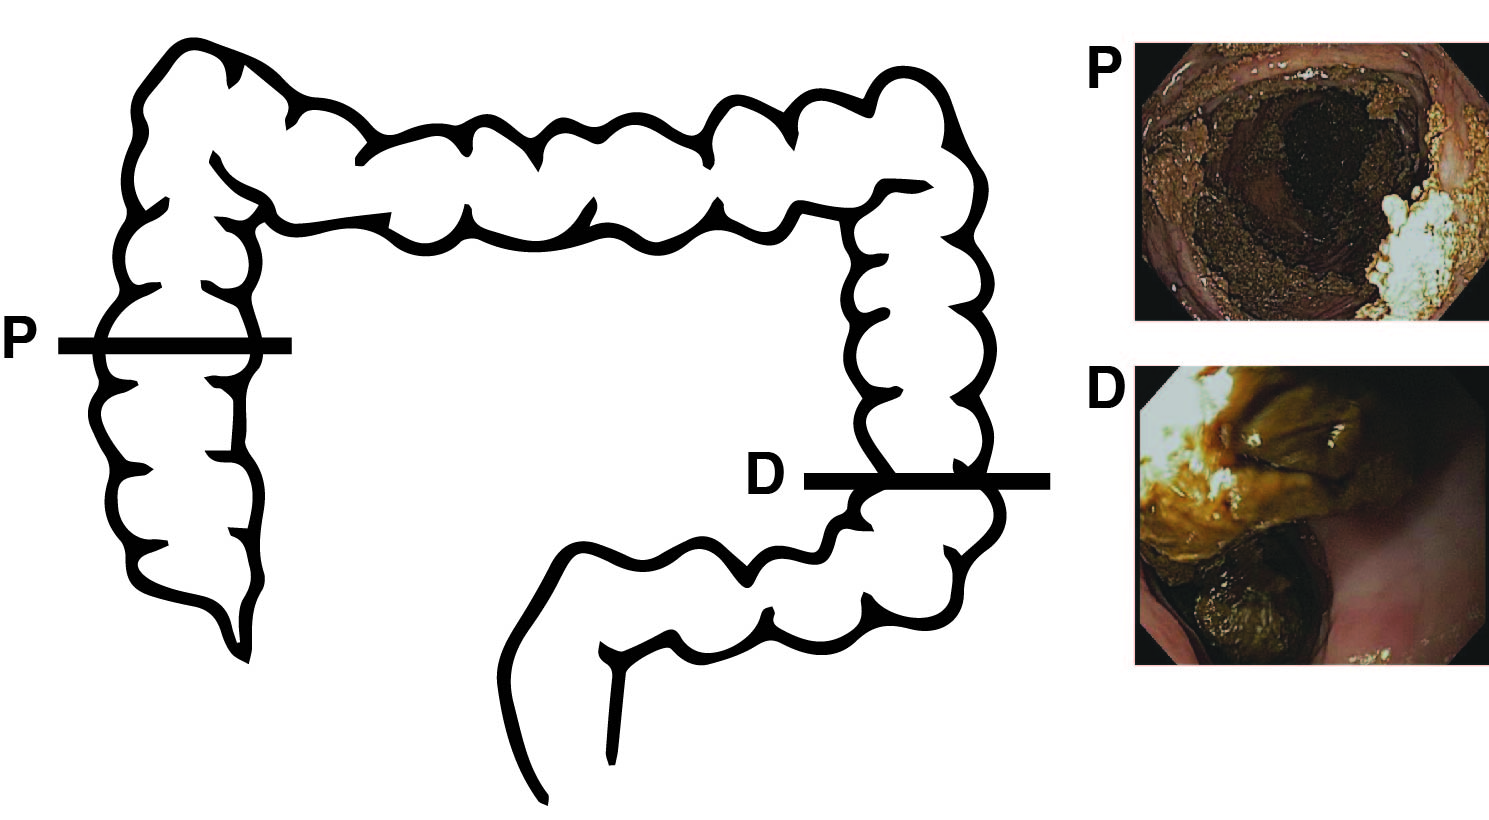
\includegraphics{../submission/fig1.jpg}
\caption{Fig 1}
\end{figure}

\newpage

\paragraph{Figure 2}\label{figure-2}

Phylum-level relative abundance and diversity in the proximal and distal
human colon. A) Relative abundance of the top five bacterial phyla in
each sampling site. Each box represents the median and interquartile
range. B) Simpson diversity of the microbial communities at each
location. The horizontal lines represent the median values.

\begin{figure}[htbp]
\centering
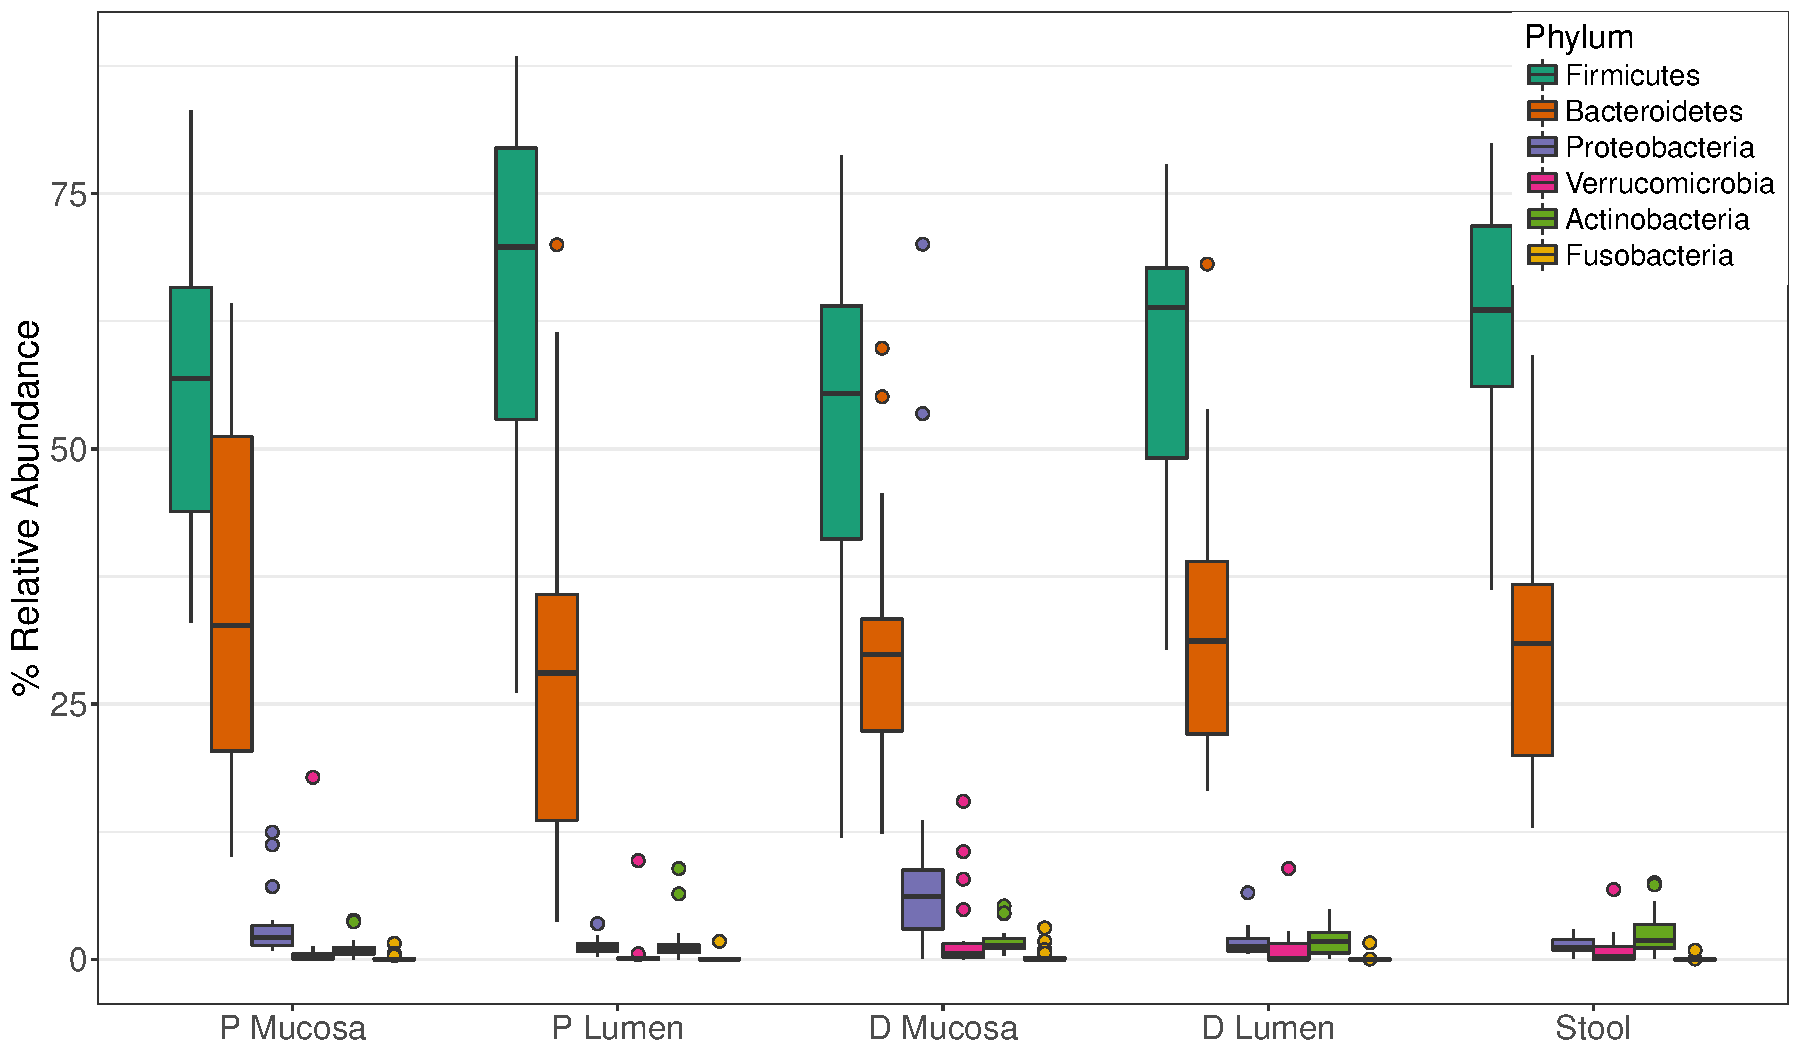
\includegraphics{../submission/figure_2.pdf}
\caption{Fig 2}
\end{figure}

\newpage

\paragraph{Figure 3}\label{figure-3}

Comparison of microbial community structure between sites of the gut.
\(\theta\)YC distances are shown to indicate the interpersonal
dissimilarities between two sites -- each point represents one
individual. In (A), comparisons of the proximal and distal mucosal and
lumen are shown. In (B), comparisons of each site to the exit stool are
shown. In (C), comparisons of samples from all subjects to each other
(interpersonal) or within one subject (intrapersonal) are shown.

\begin{figure}[htbp]
\centering
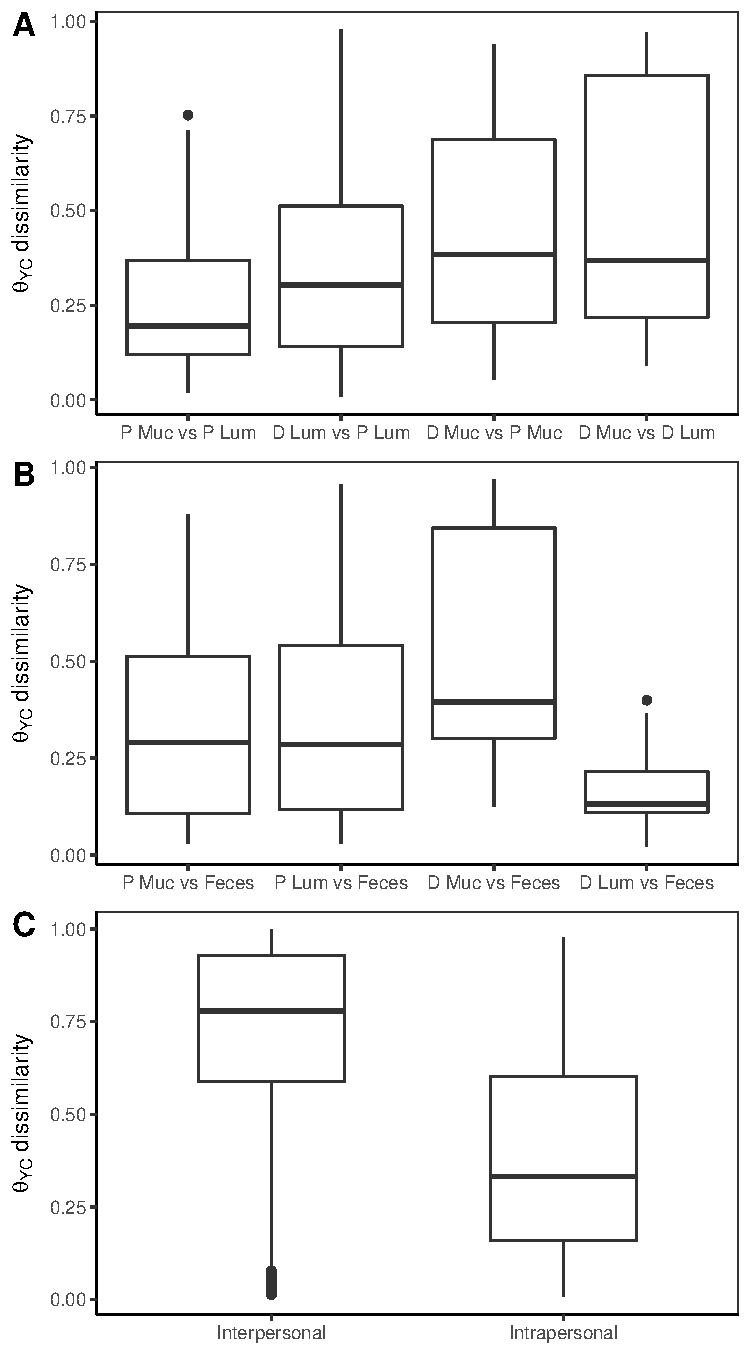
\includegraphics{../submission/figure_3.pdf}
\caption{Fig 3}
\end{figure}

\newpage

\paragraph{Figure 4}\label{figure-4}

Random Forest classifies locations in the colon. A) Receiver Operator
Characteristic curves are shown for the 10-fold cross validation of the
Random Forest model classifying lumen and mucosal samples for the distal
(red) and proximal (blue) sides of the colon. (B) Receiver Operator
Characteristic curves are shown for the 10-fold cross validation of the
Random Forest model classifying distal mucosa vs proximal mucosa (green)
and distal lumen versus proximal lumen (purple).

\begin{figure}[htbp]
\centering
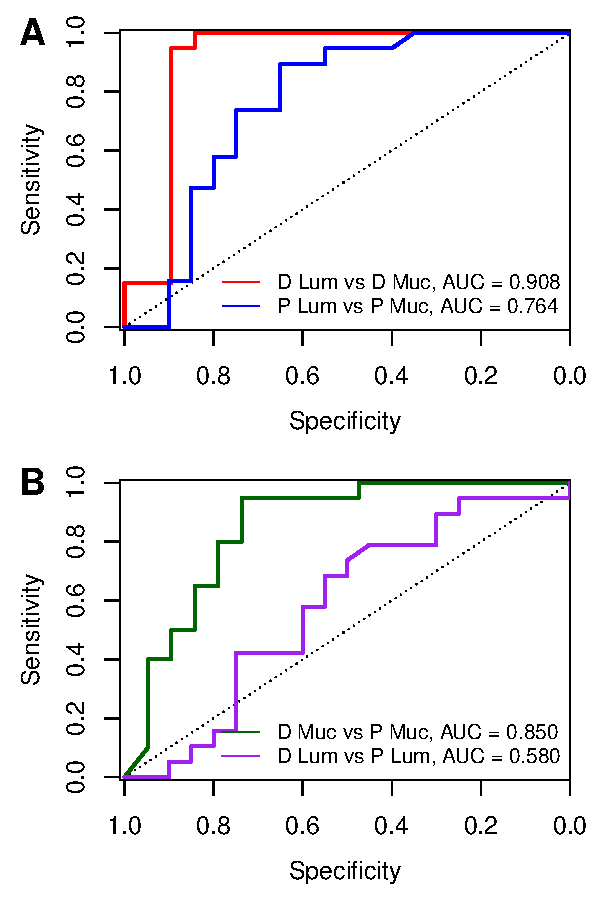
\includegraphics{../submission/figure_4.pdf}
\caption{Fig 4}
\end{figure}

\newpage

\paragraph{Figure 5}\label{figure-5}

Taxa specific to the distal and proximal sides of the colon. Top five
OTUs that are most important for the classification model for the distal
mucosa and lumen (A) and the proximal mucosa and lumen (B). The vertical
lines represent the median values for each OTU.

\begin{figure}[htbp]
\centering
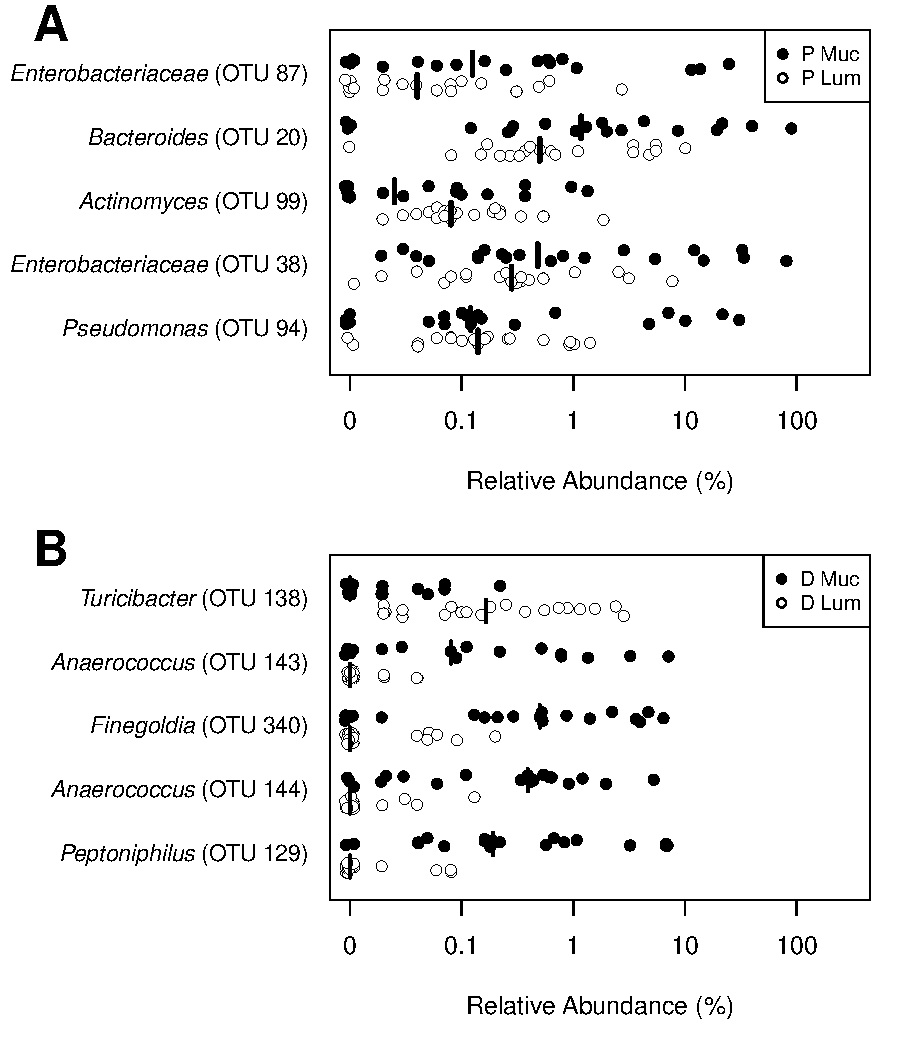
\includegraphics{../submission/figure_5.pdf}
\caption{Fig 5}
\end{figure}

\newpage

\paragraph{Figure 6}\label{figure-6}

Taxa specific to the distal and proximal mucosa and lumen. The five OTUs
that were most important differentiating the distal and proximal mucosa
(A) and the distal and proximal lumen (B). The vertical lines represent
the median values for each OTU.

\begin{figure}[htbp]
\centering
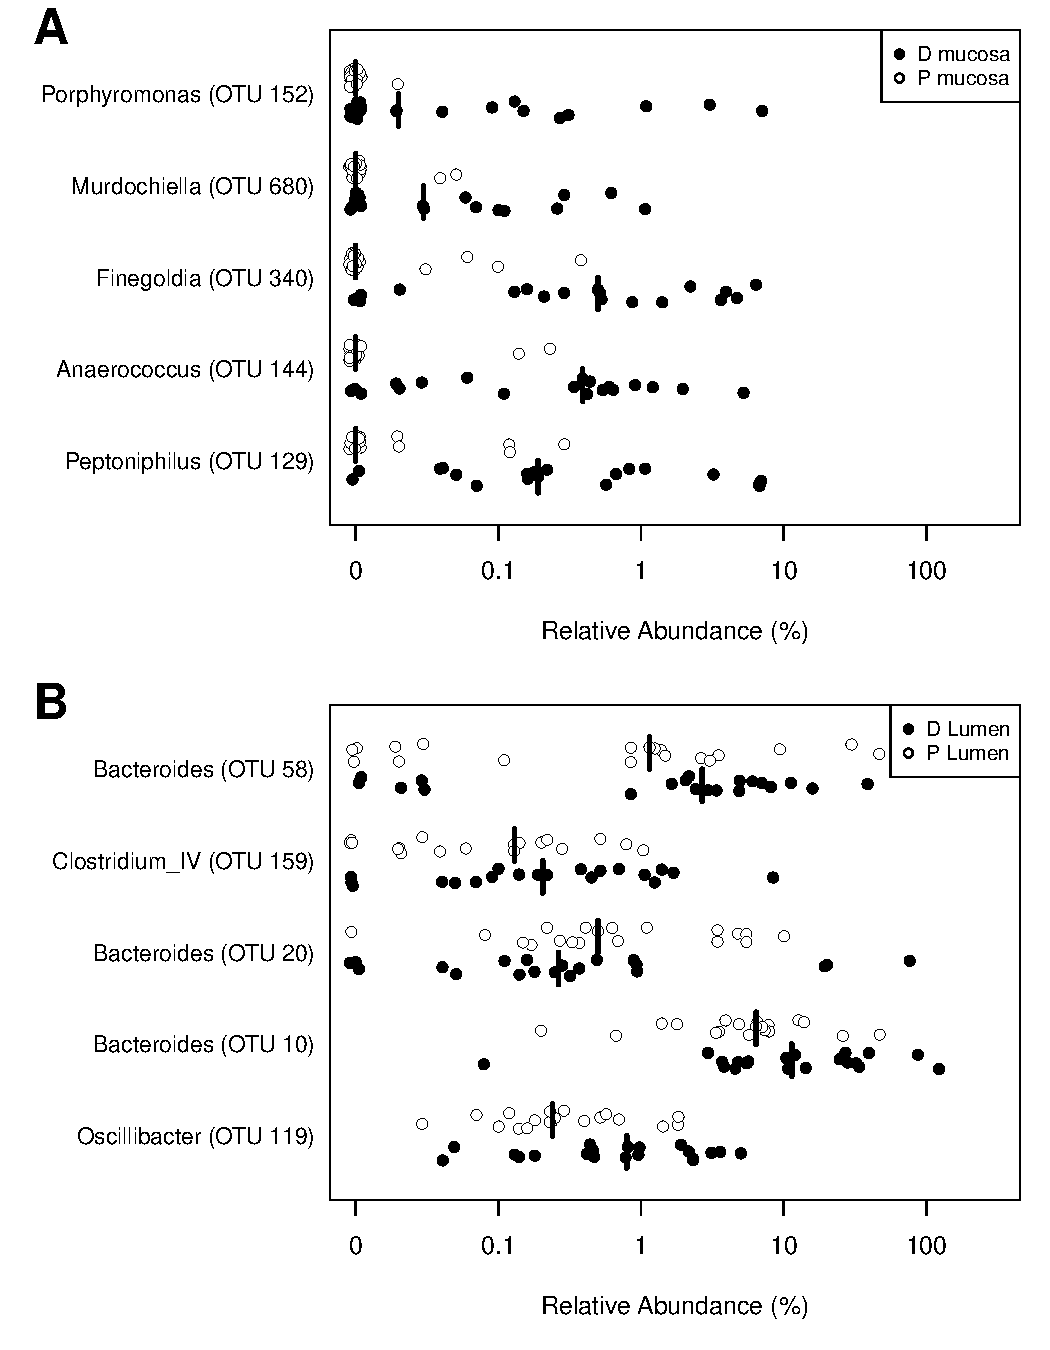
\includegraphics{../submission/figure_6.pdf}
\caption{Fig 6}
\end{figure}

\newpage

\paragraph{Figure S1}\label{figure-s1}

Location and relative abundance of cancer-associated OTUs. Relative
abundance was calculated and plotted by sample site for each OTU of
interest: (A) \emph{Fusobacterium nucleatum subsp. animalis} (B)
\emph{Fusobacterium varium} and (C) \emph{Porphyromonas asacharolytica}
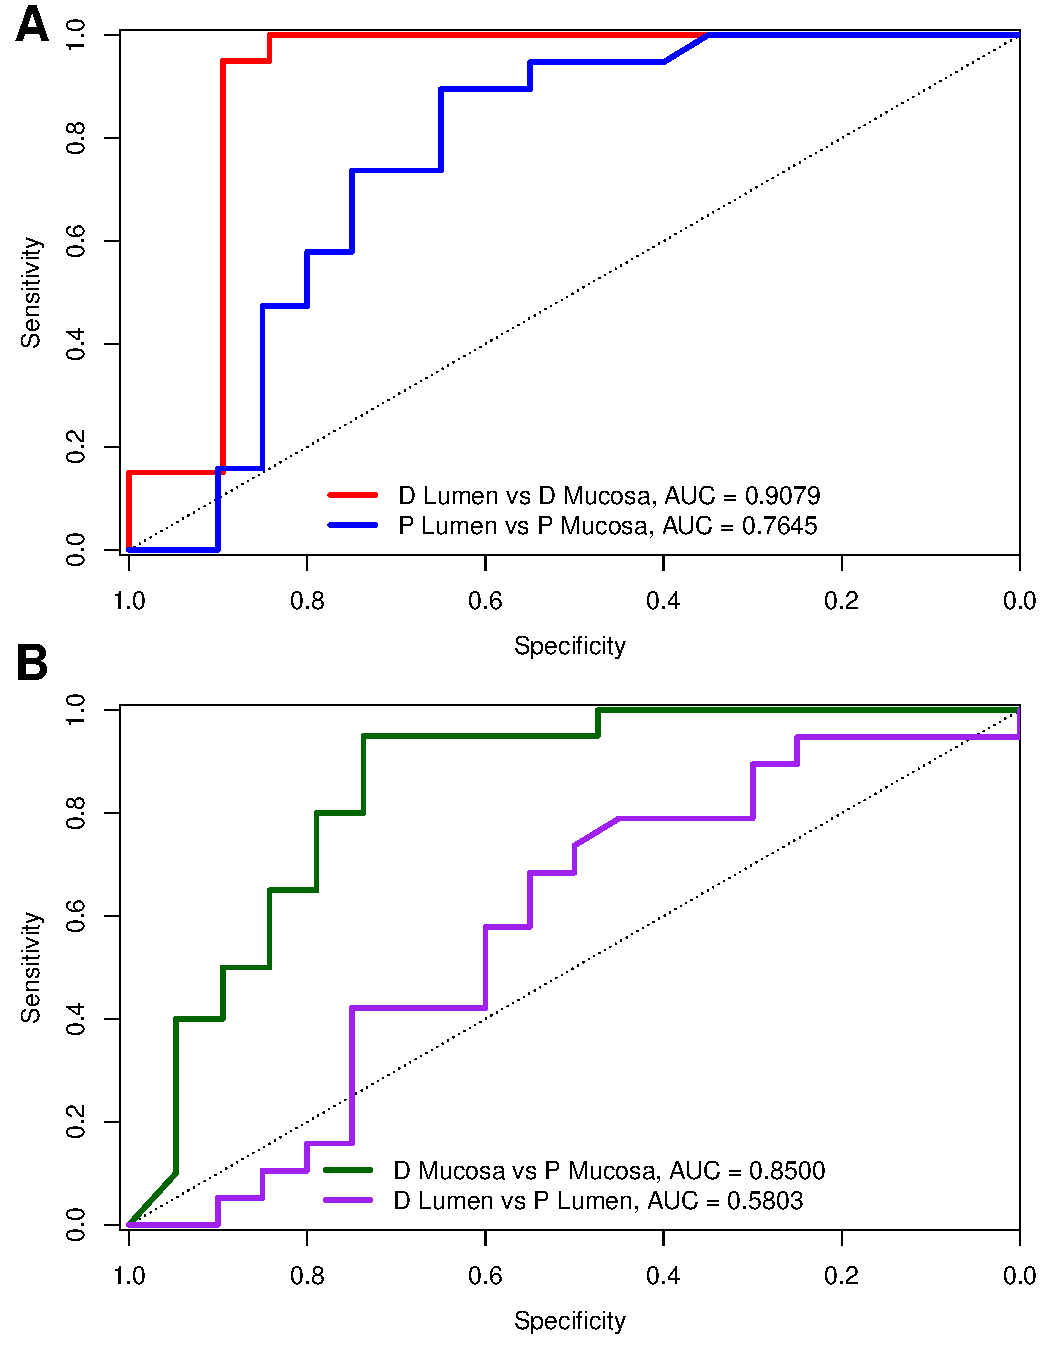
\includegraphics{../submission/figure_S1.pdf}

\newpage


\end{document}
